\subsection{FUNCTORIAL PROPERTIES OF THE SYMMETRIC ALGEBRA}

PROPOSITION 3. Let A be a commutative ring, M and N two A-modules and u: M → N an A-linear mapping. There exists one and only one A-algebra homomorphism \(u'\) : S(M) → S(N) such that the diagram

\pandocbounded{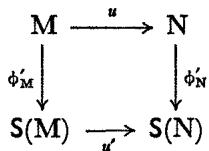
\includegraphics[keepaspectratio]{images/part003_0f38c769.jpg}}

is commutative. Moreover, \(u'\) is a graded algebra homomorphism.

The existence and uniqueness of \(u'\) follow from no. 1, Proposition 2 applied to the commutative algebra \(\mathbf{S}(\mathbf{N})\) and \(f = \phi_{\mathbf{N}}' \circ u: \mathbf{M} \to \mathbf{S}(\mathbf{N})\) ; as

\[
f (\mathbf {M}) \subset \mathbf {S} ^ {1} (\mathbf {N}) = \mathbf {N},
\]

the fact that \(u'\) is a graded algebra homomorphism follows from no. 1, Remark 1.

The homomorphism \(u'\) of Proposition 3 will henceforth be denoted by \(S(u)\) . If \(P\) is an A-module and \(v: N \to P\) an A-linear mapping, then

\[
\mathbf {S} (v \circ u) = \mathbf {S} (v) \circ \mathbf {S} (u)\tag{3}
\]

for \(\mathbf{S}(v) \circ \mathbf{S}(u)\) is an algebra homomorphism rendering commutative the diagram

\pandocbounded{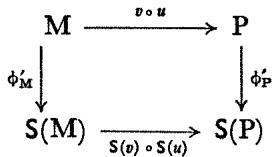
\includegraphics[keepaspectratio]{images/part003_67e6d402.jpg}}

As \(\mathbf{S}(\mathbf{M})\) contains \(\mathbf{M} = \mathbf{S}^1 (\mathbf{M})\) , \(\mathbf{S}(u)\) is sometimes called the canonical extension of \(u\) to \(\mathbf{S}(\mathbf{M})\) . The restriction \(\mathbf{S}^n (u): \mathbf{S}^n (\mathbf{M}) \to \mathbf{S}^n (\mathbf{N})\) is such that

\[
\mathsf {S} ^ {n} (u) \left(x _ {1} x _ {2} \dots x _ {n}\right) = u \left(x _ {1}\right) u \left(x _ {2}\right) \dots u \left(x _ {n}\right)
\]

where the \(x_{i} \in M\) , since \(\mathbf{S}(u)\) is an algebra homomorphism and \(\mathbf{S}^{1}(u) = u\) ; the restriction \(\mathbf{S}^{0}(u)\) to A is the identity mapping. Note that \(\mathbf{S}^{n}(u)\) can be obtained from \(\mathbf{T}^{n}(u): \mathbf{T}^{n}(\mathbf{M}) \to \mathbf{T}^{n}(\mathbf{N})\) by passing to the quotients.

PROPOSITION 4. If \(u: \mathbf{M} \to \mathbf{N}\) is a surjective A-linear mapping, the homomorphism \(\mathbf{S}(u): \mathbf{S}(\mathbf{M}) \to \mathbf{S}(\mathbf{N})\) is surjective and its kernel is the ideal of \(\mathbf{S}(\mathbf{M})\) generated by the kernel \(\mathbf{P} \subset \mathbf{M} \subset \mathbf{S}(\mathbf{M})\) of \(u\) .

We write \(v = \mathsf{T}(u) \colon \mathsf{T}(\mathbf{M}) \to \mathsf{T}(\mathbf{N})\) ; we know (§ 5, no. 2, Proposition 3) that \(v\) is surjective and hence it follows from the definitions that \(v(\mathfrak{J}_{\mathbf{M}}') = \mathfrak{J}_{\mathbf{N}}'\) ; if \(\Re\) is the kernel of \(v\) , then \(v^{-1}(\mathfrak{J}_{\mathbf{N}}') = \Re + \mathfrak{J}_{\mathbf{M}}'\) . As \(\mathsf{S}(u) \colon \mathsf{T}(\mathbf{M}) / \mathfrak{J}_{\mathbf{M}}' \to \mathsf{T}(\mathbf{N}) / \mathfrak{J}_{\mathbf{N}}'\) is derived from \(v\) by passing to the quotients, it is a surjective homomorphism whose kernel is \(\Re' = (\Re + \mathfrak{J}_{\mathbf{M}}') / \mathfrak{J}_{\mathbf{M}}'\) . As \(\Re\) is generated by the kernel \(\mathbf{P}\) of \(u\) (§ 5, no. 2), so is \(\Re'\) .

If \(u: \mathbf{M} \to \mathbf{N}\) is an injective linear mapping, it is not always true that \(\mathbf{S}(\mathbf{u})\) is an injective mapping (Exercise 1). However it is so when \(u\) is an injection such that \(u(\mathbf{M})\) is a direct factor in \(\mathbf{N}\) and then the image of \(\mathbf{S}(u)\) (isomorphic to \(\mathbf{S}(\mathbf{M})\) ) is a direct factor of \(\mathbf{S}(\mathbf{N})\) ; the proof is the same as that for the analogous assertions for \(\mathbf{T}(u)\) ( \(\S 5\) , no. 2) replacing \(\mathbf{T}\) by \(\mathbf{S}\) .

PROPOSITION 5. Let N and P be two submodules of an A-module M such that their sum \(N + P\) is a direct factor in M and their intersection \(N \cap P\) is a direct factor in N and in P. Then the homomorphisms \(\mathsf{S}(\mathsf{N}) \to \mathsf{S}(\mathsf{M}), \mathsf{S}(\mathsf{P}) \to \mathsf{S}(\mathsf{M})\) and

\[
\mathbf {S} (\mathbf {N} \cap \mathbf {P}) \rightarrow \mathbf {S} (\mathbf {M}),
\]

canonical extensions of the canonical injections, are injective; if \(\mathbf{S}(\mathbf{N})\) , \(\mathbf{S}(\mathbf{P})\) and \(\mathbf{S}(\mathbf{N} \cap \mathbf{P})\) are identified with subalgebras of \(\mathbf{S}(\mathbf{M})\) by means of these homomorphisms, then

\[
\mathbf {S} (\mathbf {N} \cap \mathbf {P}) = \mathbf {S} (\mathbf {N}) \cap \mathbf {S} (\mathbf {P}).\tag{4}
\]

The proof reduces to that of § 5, no. 2, Proposition 4 replacing T by S throughout. The hypotheses of Proposition 5 always hold for arbitrary submodules N, P of M when A is a field.

COROLLARY. Let K be a commutative field and M a vector space over K. For every element \(z \in \mathbb{S}(\mathbf{M})\) there exists a smallest vector space N of M such that \(z \in \mathbb{S}(\mathbf{N})\) and N is finite-dimensional.

The proof is derived from that of § 5, no. 2, Corollary to Proposition 4 replacing T by S throughout.

N is called the vector subspace of M associated with z.

